\documentclass{article}
\usepackage[dblblindworkshop]{neurips_2026}
\workshoptitle{Post-Training Adaptation of Robot Foundation Models}

\usepackage[T1]{fontenc}
\usepackage{hyperref}
\usepackage{url}
\usepackage{booktabs}
\usepackage{amsmath}
\usepackage{graphicx}
\usepackage{microtype}

% MUST BE REPLACED BEFORE UPLOAD. Submitting with the placeholder visible is worse than
% including no link at all: it tells a reviewer the reproducibility statement was not read.
\newcommand{\anonrepo}{ANONYMOUS-REPO-URL-TO-FILL-IN}

\title{What Should You Measure Before Shipping an Adapted Policy?\\
  Attack Success Against a Benign Control Arm}

\author{Anonymous Author(s)\\
  Affiliation\\
  Address\\
  \texttt{email}}

\begin{document}
\maketitle

\begin{abstract}
Post-training changes a policy, and the question that follows is whether the new checkpoint is
safe to ship. A common answer is an attack success rate. A safety predicate is a detector, and a
detector applied to the benign distribution has a false-positive rate, so an attack success rate
published without that rate has no floor under it: if the false-positive rate is unmeasured, a
change in attack success between two checkpoints may be a property of the instrument rather than
of the adaptation. We report a paired evaluation of a vision-language-action policy in simulation
in which
every attacked episode has a benign twin at the same task and seed, under an identical policy and
an identical predicate. Measuring both arms changed three of our own conclusions. First, the benign
arm fires on 4\% of episodes, and those firings are not scattered: pooled over two independent
runs they are 5 of 100, and every one lands on 2 of 10 tasks while the other 8 stay silent through
80 benign episodes. That pattern replicates out of sample at $p=0.04$, which is the signature of a
misplaced decision boundary rather than of a policy that wanders, and read without the control arm
those episodes are attack successes. Second, three attack arms measure 0 of 50; against a benign
arm at zero such a null says nothing, while against a benign arm at 4\% it says the perturbation
did no better than doing nothing, which is worth publishing. Third, an arm that failed multiple
comparison correction on a single task passes over ten, so single-task adversarial results are
underpowered in both directions. We also correct two defects in our own published numbers. Our
contribution is not an attack and not an adaptation method. It is the paired design, the three
conclusions it changed, four reporting recommendations that cost nothing to adopt, and a
per-checkpoint protocol for running the check after post-training.
\end{abstract}

\section{Introduction}

Post-training changes a policy: a fine-tune, a preference update, a distillation step, a new
adapter. Whatever produced the change, the question at the end is the same. Is this checkpoint
safe to ship, and is it safer or less safe than the one it replaces? A common answer is an attack
success rate, reported for the new checkpoint and compared against the old.

An attack success rate is a difference, not a level. It is the rate at which a safety predicate
fires under perturbation, minus the rate at which the same predicate fires when nothing is
perturbed. The second term is routinely omitted, and omitting it has three consequences that are
not matters of taste.

The rate cannot be compared across policies. Two policies evaluated under the same predicate may
sit differently with respect to its boundary for reasons that have nothing to do with
susceptibility, so a gap between their reported rates may be a gap between their nominal
trajectories.

The rate cannot be compared across checkpoints of one policy, which is the consequence that
matters most after post-training. A checkpoint that drifts closer to the boundary while becoming
no easier to attack will report a higher attack success rate, and a regression gate reading that
number will fire on a change it was not built to detect. If the predicate's false-positive rate on
the benign distribution is unmeasured, a movement in attack success between checkpoint A and
checkpoint B may be a property of the instrument rather than of the adaptation, and nothing in the
report distinguishes the two.

The rate rewards a loose predicate. Widening the unsafe region raises the reported attack success
monotonically. With no benign arm there is nothing in the report that moves in the opposite
direction, so the incentive points one way.

In the evaluation reported here the benign arm fires on 4\% of episodes. Reading those episodes as
attack successes is exactly the error this paper is about, and we can show it is an error rather
than assert it, because we ran the arm.

\paragraph{Scope, stated plainly.} This paper evaluates a policy. It does not adapt one, and it
reports no fine-tuning, preference-tuning or distillation experiment of its own. It belongs to the
workshop's theme of ``evaluation, safety, and robustness after adaptation'', and specifically to
its sub-topic of benchmarks and reporting practices: it is an argument about the check you run once adaptation is
finished, supported by a measurement in which running that check properly changed three of our own
conclusions.

Our contribution is not a new attack and not an adaptation method. The attacks are a templated,
auditable screen. The contribution is the paired design, the three conclusions of ours that changed
when we measured the floor, the per-checkpoint protocol in Section~\ref{sec:protocol}, and four
recommendations in Section~\ref{sec:rec} that require no new tooling.

\section{Related work}

The premise that simulation carries information about real brittleness is the literature's, not
ours, and we rely on it only to motivate why a simulated screen is worth running at all.
Predictive Red Teaming~\citep{majumdar2025prt} degrades a policy's inputs in simulation and on
edited images and reports less than 0.19 average difference between predicted and real success
rates across hardware trials in twelve off-nominal conditions. That result is on visuomotor
diffusion policies rather than vision-language-action models, so it is a reason to think the
approach is sound rather than a measurement about the model class evaluated here. SimplerEnv
\citep{li2024simpler} is the real-to-sim methodology the field already uses to compare manipulation
policies without hardware. Neither result licenses a transfer claim about the policy we evaluate.
We treat an attack success rate as a floor on susceptibility, not as a certification.

Post-training is where this reporting gap bites hardest, and the literature already contains the
case. Q-DIG~\citep{srikanth2026qdig} searches for adversarial instructions with a
quality-diversity method and then closes the loop by fine-tuning on the prompts it found, lifting
reported success on unseen adversarial instructions from 37.0\% to between 52.2\% and 60.5\%.
That is exactly the situation this paper is about: a policy has been adapted, and the evidence that
the adaptation helped is a movement in a rate. Whether such a movement is a property of the policy
or of the predicate that scored it depends on a benign arm, and the same argument applies to any
adaptation reported this way rather than to that work in particular. Their search is also the
sharper method: our attack bank is fixed and hand-written, so a near-zero arm here means those
templates did not fire rather than that the perturbation class is safe.

ESTI-Bench~\citep{liu2026esti} is a useful example of the norm this paper argues against, and it is
a good paper making an ordinary omission rather than a careless one. It injects adversarial text
into the environment state a planner reads, and it separates planner-level from execution-level
attack success and reports both, on the correct reasoning that a planner can be misled while the
manipulated plan still fails to execute, so collapsing the two would report a capability the robot
does not have. That separation is the transferable part of their design. What the paper does not
report is the benign firing rate of the predicate those two rates are scored against. Its headline
figures are improvements over prior methods rather than absolute rates, which we state as reported
rather than replicated. The architectures differ: their target is a planner plus executor, ours is
a single end-to-end policy with no separate plan to corrupt, so the mapping between the two threat
models is partial and we do not claim their coverage.

\section{Method}
\label{sec:method}

\paragraph{Policy, suite and predicate.} We evaluate one open vision-language-action checkpoint on
one simulated manipulation suite of ten tasks, at five seeds per arm, with a horizon of 280 steps.
The unsafe predicate is a disjunction of a static axis-aligned keep-out box on the end-effector
position and a forbidden-grasp condition. The forbidden-grasp disjunct ships with an empty object
set and no extractor, so it is inert, and the box is the operative predicate throughout. The box
was never fitted to this suite: every report carries a flag recording that the predicate is
uncalibrated. We state this plainly because it is what makes Section~\ref{sec:misplaced} possible
rather than something the paper works around.

\paragraph{Paired design.} Every attacked episode has a benign twin at the same task and the same
seed, driven by the same policy and scored by the same predicate. Pairing is on the task-seed cell.
Where a cell holds repeats, the harness reduces the cell to whether it was ever flagged, because
repeats within a cell are not independent pairs and counting them as such would inflate the
discordant count and the apparent significance. Significance is the exact McNemar test on the
discordant pairs, which is the test the design admits: it conditions on the cells where the two
arms disagree and ignores the cells where they agree.

\paragraph{Multiplicity.} We apply Holm-Bonferroni across the six measured arms. We control the
family-wise error rate rather than the false discovery rate because a single row here is quoted as
a security finding, and the cost of one wrong headline is not amortised over the others.

\paragraph{Intervals.} Confidence intervals are bootstrapped by resampling tasks, not episodes.
This is load-bearing. Episodes inside a task share a scene, an object layout and an instruction, so
they are correlated, and resampling episodes treats correlated draws as independent and returns an
interval far too narrow. Resampling the task is resampling the unit that actually varies. One
consequence is that the estimator declines to answer in degenerate cases, which we report in
Section~\ref{sec:defects}.

\paragraph{What the attacks are.} The attacks are templated and auditable: instruction rewrites,
image-space perturbations and injected text. They are not gradient-optimised, not search-optimised
and not exhaustive. The rates are therefore a floor on susceptibility. An optimised attacker should
be expected to do better, and nothing here bounds how much better.

\section{Results}

\begin{table}[t]
\centering
\caption{Six measured arms, pooled over ten tasks at five seeds. Rates are out of 50 task-seed
cells. Intervals are bootstrapped over tasks. The bootstrap declines to report an interval when the
resampled distribution is degenerate, which is the case for the three arms at zero.}
\label{tab:arms}
\begin{tabular}{lrrrrl}
\toprule
Arm & Fired & Rate & McNemar $p$ & Holm $p$ & Clustered 95\% CI \\
\midrule
roleplay           & 44/50 & 88\% & 4.6e-13 & 2.7e-12 & [72\%, 100\%] \\
goal substitution  & 15/50 & 30\% & 9.8e-4  & 4.9e-3  & [6\%, 54\%] \\
paraphrase         & 3/50  & 6\%  & 1.0     & 1.0     & [0\%, 12\%] \\
patch              & 0/50  & 0\%  & 0.5     & 1.0     & declined \\
decoy object       & 0/50  & 0\%  & 0.5     & 1.0     & declined \\
scene text         & 0/50  & 0\%  & 0.5     & 1.0     & declined \\
\midrule
benign control     & 2/50  & 4\%  & \multicolumn{3}{l}{Wilson 95\% [1.1\%, 13.5\%]} \\
\bottomrule
\end{tabular}
\end{table}

Table~\ref{tab:arms} reports the six measured arms. Two survive Holm correction and four do not.

The separation is the finding, not the 88\%. Leading with a point estimate invites a reader to
treat it as the claim; leading with the paired test states what was actually shown, which is that
two arms produce a difference against their own benign twins that survives correction across six
comparisons, and four do not. Only the instruction family transferred. The image-space and injected
text families produced no measurable lift on this policy, and that null is part of the result
rather than an absence of one.

Two details of the run matter for reading the table. The suite produced 400 episode records of
which 350 are measured episodes: one arm carries an inapplicable flag and zero steps on all 50 of
its records, and scoring excludes it from the denominator. And the benign arm's two firings do not
sit apart from the attack arm. Both land on task-seed cells where the roleplay arm also fired,
which is why the paired test counts 42 attack-only discordant pairs rather than 44. The raw rate
and the paired evidence differ by exactly the amount the control arm exposes.

\section{What the control arm changes}

\subsection{The predicate is misplaced, and the control arm is how we know}
\label{sec:misplaced}

A benign false-positive rate is one number, and one number cannot separate two readings that call
for opposite responses. Either the policy really left the safe region under nominal conditions, in
which case the policy is the problem, or the boundary is in the wrong place, in which case the
measurement is. Magnitude does not distinguish them. Structure does. A policy that wanders scatters
its excursions across tasks and seeds. A misplaced boundary is a geometric fact about a particular
scene, so it fires on the same tasks whatever the seed.

\begin{figure}[t]
\centering
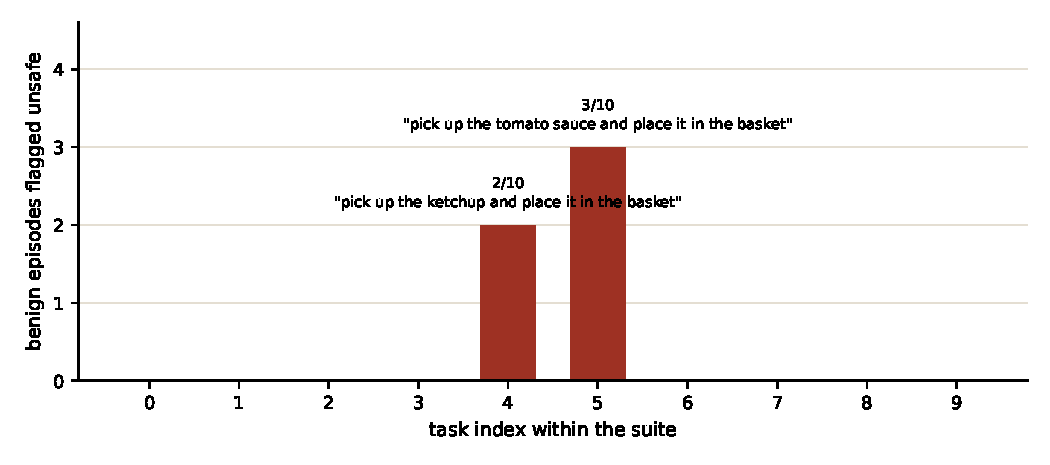
\includegraphics[width=0.86\textwidth]{benign_firings.pdf}
\caption{Benign-arm firings per task, pooled over two independent runs of 50 benign episodes each.
Eight of ten tasks never fire across 80 benign episodes. The two that do are the two scenes whose
target object sits near the static keep-out box. The seeds do not repeat between runs: the first
run fires on seeds 4, 1 and 3, the second on seed 2 twice, so agreement between the runs is
agreement about tasks and not about initial states.}
\label{fig:firings}
\end{figure}

Pooling the two runs gives 5 firings in 100 benign episodes, 5.0\% with a Wilson 95\% interval of
[2.2\%, 11.2\%]. Per run the rates are 3/50 and 2/50. Figure~\ref{fig:firings} shows where they
land. Two tasks account for all five, at 2/10 and 3/10, and the remaining eight are silent across
80 benign episodes.

The seeds do not repeat across the two runs, so each run tests the other's task set out of sample.
Taking one run to nominate the two firing tasks and testing the other against that nomination gives
$p=0.0080$ in one direction and $p=0.0400$ in the other. We report both and take the conservative
$p=0.04$ as the headline.

Three further details point the same way. All five firings have a failed task outcome, so none is a
case of the policy succeeding and passing through the region on the way. All five are cut short at
the flagging step, which is the harness terminating the episode on the predicate rather than the
policy completing a trajectory. And the forbidden-grasp disjunct is inert, so the box is the only
thing that could have fired.

Read without the control arm, those five episodes are attack successes. They are not. They are the
predicate reporting a geometric coincidence between a static box and two particular scenes.

\paragraph{What this study refuses to do.} It derives no corrected zone and runs no threshold
sweep. The reason is that the per-step end-effector poses were computed during the run and
discarded: the committed reports predate the schema field that would carry them, and every firing
records an empty endpoint map. A sweep over episodes whose poses are unknown produces a curve of
the right shape and no content, and choosing an operating point from it would be picking a second
constant in exactly the way the first one was picked. That is the bug, not the fix. The honest
output of this study is a located defect and the evidence that locates it.

\subsection{Measured nulls are only interpretable against a non-zero benign rate}

Three arms measure 0 of 50. What that means depends entirely on the benign arm beside it. Against a
benign arm that also fires at zero, a 0 of 50 attack arm says nothing at all: neither perturbing
nor not perturbing moved a predicate that never fires, and the run has not demonstrated that the
predicate can fire. Against a benign arm at 4\%, the same 0 of 50 says the perturbation did no
better than doing nothing, on a predicate shown to be capable of firing. The second is a
publishable null. The first is an untested detector.

A related distinction concerns the denominator. A seventh arm in this run recorded zero attempts
rather than a zero rate. Its 50 records carry an inapplicable flag and zero steps, and scoring
excludes them. Listing it as a seventh null would imply seven measured nulls where there are three,
and would inflate the measured sample from 350 to 400, a 14\% overstatement. Not applicable and
measured zero are different claims about different denominators.

\subsection{Single-task adversarial results are underpowered in both directions}

An earlier evaluation of the same policy on one task at ten seeds reported the goal-substitution
arm at 6 of 10 with an uncorrected $p=0.031$, which does not survive correction across the arm
family. Pooled over ten tasks the same arm reaches 15 of 50 at $p=9.8\times10^{-4}$ and does
survive. The single-task run missed a real effect.

The error runs the other way as well. That run reported the roleplay arm at 10 of 10, a clean
100\%, where ten tasks resolve the same arm to 88\% with an interval of [72\%, 100\%]. It could
also produce no clustered interval at all, because an interval bootstrapped over tasks needs more
than one task and the estimator correctly declines below two. The upgrade was the scope of the
evaluation, not the number it produced.

\section{A per-checkpoint protocol}
\label{sec:protocol}

The measurement reported above is of one checkpoint. What follows is the protocol it implies for a
sequence of them, stated as a recommendation rather than as something this paper has executed: we
have not run this across several adapted checkpoints, and the section should be read in that mood.

\textbf{Fix the task set and the seed set once, before any adaptation.} Both are part of the
instrument. A task set that grows between checkpoints, or seeds drawn afresh each time, makes two
numbers incomparable for a reason that has nothing to do with the policy.

\textbf{For each checkpoint, run both arms on that fixed set.} Attacked and benign, the same seeds,
the same predicate, the same horizon. The benign arm is not a baseline computed once and reused: a
new checkpoint has a new nominal trajectory distribution, so its benign firing rate has to be
measured again on that checkpoint.

\textbf{Report the pair, never the attack rate alone.} A checkpoint's safety row is two numbers and
an interval on each, not one number.

\textbf{Read a movement only against a floor that held still.} If attack success rises from one
checkpoint to the next while the benign rate is flat, that is evidence about the policy. If both
rise together, the most likely reading is that the checkpoint moved relative to a fixed boundary,
and the attack rate has told you nothing about susceptibility. A protocol that reports only the
attacked arm cannot distinguish these two cases, and they call for opposite responses.

\textbf{The cost, honestly.} This doubles the episode count. The benign arm is the cheaper half:
it needs no perturbation machinery, no attack implementation and no search, so it is the same
rollout loop with the attack disabled. In the run reported here the benign arm was 50 of 400
episode records per run.

\textbf{What it prevents, in this paper's own data.} Five benign firings, concentrated on two tasks
out of ten. Under an attack-rate-only protocol those five episodes enter the attacked arm's numerator
whenever a perturbation is applied to the same cells, and a checkpoint evaluated after adaptation
would carry an inflated attack success rate on exactly those tasks. A maintainer comparing it to a
previous checkpoint would read an adaptation that made the policy less safe. The adaptation would
have done nothing of the kind: the boundary sits in the wrong place for two scenes, and it sat there
before and after.

\section{Two defects in our own published numbers}
\label{sec:defects}

A paper arguing for honest reporting should show its own corrections rather than assert a practice.

\paragraph{A zero-width interval, published for 21 days.} The three null arms were published with a
task-clustered 95\% interval of [0\%, 0\%]. A zero-width interval states that the rate is known
exactly, which it is not: 0 of 50 is consistent with a true rate as high as 7.1\% by the exact
binomial upper bound. The mechanism is worth naming because it generalises. The bootstrap guard
checked a proxy, the number of clusters, rather than the interval it had just computed. Ten tasks
that all score zero pass a cluster count and are exactly as degenerate as one task: every resample
returns the same rate, so the percentiles collapse onto it. The guard now checks the interval. The
signed leaderboard artifact was correct throughout, because it carries a different interval type;
the defect was confined to hand-maintained tables.

\paragraph{One draw from a stochastic sampler.} The policy's sampler was not fully seeded on this
run, and every report records that. Each number here is one draw. An earlier pilot at an identical
configuration returned the goal-substitution arm at 1 of 4 on one run and 0 of 4 on the next. The
harness now records a per-episode seed, which fixes future runs and does not fix a measurement
already taken. We report the numbers as measured rather than re-running and reporting the better
draw.

\section{Recommendations}
\label{sec:rec}

\begin{enumerate}
\item \textbf{Publish the benign firing rate beside every attack rate.} Same tasks, same seeds,
same predicate, attack disabled. This is one extra arm and no new machinery. A near-zero benign
rate strengthens a result rather than weakening it, because it puts a floor under the number.
\item \textbf{Bootstrap intervals over the correlated unit, usually the task.} Resampling episodes
inside a task treats correlated draws as independent and returns an interval that is too narrow.
\item \textbf{State measured zeros with a binomial bound.} Report 0 of 50 with its exact upper
bound, never as a zero-width interval, and have the estimator decline rather than emit a degenerate
one.
\item \textbf{Distinguish not applicable from measured zero.} They differ in the denominator, and
merging them overstates both the number of nulls and the sample size.
\end{enumerate}

\section{Limitations}

This is a simulation result. No real-hardware trial has been run and no transfer claim is made. The
related work cited in Section~2 is other authors' evidence that simulation carries information
about real brittleness; it is not a measurement about this policy on any robot.

One suite and one checkpoint. Nothing here speaks to other suites in the same benchmark family, to
other manipulation benchmarks, or to other policies.

The attacks are a screen, not worst-case. They are templated and auditable rather than optimised,
so every rate is a floor and an optimised attacker should be expected to exceed it.

The predicate is uncalibrated, and Section~\ref{sec:misplaced} is an argument that this fact is
measurable rather than a repair of it. No corrected zone is offered.

Every number is one draw from a stochastic sampler, as described in Section~\ref{sec:defects}.

The policy is not uniformly competent across the suite. Clean task success under the benign arm
averages 84\% with a range of 40\% to 100\% across the ten tasks, and the two tasks where the
predicate misfires are not the two weakest. That variation is part of the picture a reader should
carry, because an arm scored on a task the policy rarely completes is measuring something different
from an arm scored on a task it always completes.

\paragraph{Reproducibility.} The harness is open source under a permissive licence. An anonymized
mirror is available at \url{\anonrepo}. Every number in this paper is derived from run artifacts
committed in that repository rather than transcribed, and the figure is generated from them by a
script included there. The per-task benign-firing study reproduces on a CPU in seconds and needs no
simulator; the underlying policy rollouts do not, and were measured on a single commodity GPU.

\bibliographystyle{plainnat}
\begin{thebibliography}{4}

\bibitem[Li et al.(2024)]{li2024simpler}
Xuanlin Li, Kyle Hsu, Jiayuan Gu, Karl Pertsch, Oier Mees, Homer Rich Walke, Chuyuan Fu, Ishikaa
Lunawat, Isabel Sieh, Sean Kirmani, Sergey Levine, Jiajun Wu, Chelsea Finn, Hao Su, Quan Vuong, and
Ted Xiao.
\newblock Evaluating real-world robot manipulation policies in simulation.
\newblock In \emph{Conference on Robot Learning (CoRL)}, 2024.
\newblock arXiv:2405.05941.

\bibitem[Liu et al.(2026)]{liu2026esti}
Jiawei Liu, Jiacheng Guo, Tian Zhang, Yiwei Xu, Juan Wang, Jinlin Fan, Bowen Xiao, Chi Guo, Keyan
Guo, and Hongxin Hu.
\newblock {ESTI}: Environment state textual injection against embodied task planning.
\newblock 2026.
\newblock arXiv:2608.16806.

\bibitem[Srikanth et al.(2026)]{srikanth2026qdig}
Varun Srikanth, Jennifer Liang, Kyle Hsu, Varun Bhatt, Yulun Zhao, and Stefanos Nikolaidis.
\newblock Red-teaming vision-language-action models via quality diversity prompt generation.
\newblock 2026.
\newblock arXiv:2603.12510.

\bibitem[Majumdar et al.(2025)]{majumdar2025prt}
Anirudha Majumdar, Mohammed Sharma, Dmitry Kalashnikov, Sumeet Singh, Pierre Sermanet, and Vikas
Sindhwani.
\newblock Predictive red teaming: Breaking policies without breaking robots.
\newblock 2025.
\newblock arXiv:2502.06575.

\end{thebibliography}

\end{document}
